\section{Result 1: with 8 bits per animal, no model ran out of room}\label{sec:round1}

This is the round we planned, less width 4, which learned nothing in the trial runs: the four
languages (16, 64, 256 and 1,024 animals), three widths (8, 16 and 32) and three repeats of each
pairing, 36 runs in all. Width 4 was run separately and is reported in section \ref{sec:four}.

\begin{table}[H]
\centering\small
\begin{tabular}{@{}rrrrr@{}}
\toprule
 & \multicolumn{4}{c}{Animals in the vocabulary} \\
Width & 16 & 64 & 256 & 1{,}024 \\
\midrule
8 & 100 & 100 & 100 & 100 \\
16 & 100 & 100 & 100 & 100 \\
32 & 100 & 100 & 100 & 100 \\
\bottomrule
\end{tabular}

\caption{Facts known (0 to 100) at the end of each run, with 8 bits per animal. Each entry
covers three repeats; a single number means all three gave that score.}
\label{tab:round1}
\end{table}

\textbf{All 36 runs ended as solved, with a score of 100} (table \ref{tab:round1}). A model of
width 8 learned all 4,096 facts about 1,024 animals as completely as it learned the 64 facts
about 16 animals.

Remember the catch from section \ref{sec:model}. This was not one store of fixed size taking in
64 times as much. Every added animal came with a row of its own: 8 numbers, at width 8, for an
animal with 8 bits to be remembered. The model on 1,024 animals was using all 10,936 of its
numbers; the model on 16 animals was using about 2,900. Only the body was the same in both.

\textbf{Verdict of this round: undecided}, as section \ref{sec:rule} said it would be if no
model did worse. The rule is not met for width 8 or for width 16, the two widths it could be
met for. That is not evidence against your idea, because the idea predicts a loss only once
the words no longer fit, and by the rough guide the fullest of these models (width 8 on 1,024
animals) was a little over one-third full. What the round does show is narrower: with room to
spare, 64 times as many words did not make any of these models worse.

\textbf{What a larger vocabulary did cost was training time.} Table \ref{tab:effort1} shows
how many sets each run had read when it was declared solved.

\begin{table}[H]
\centering\small
\begin{tabular}{@{}rrrrr@{}}
\toprule
 & \multicolumn{4}{c}{Animals in the vocabulary} \\
Width & 16 & 64 & 256 & 1{,}024 \\
\midrule
8 & 64, 64, 91 & 64, 91, 181 & 256, 256, 512 & 256, 512, 1{,}639 \\
16 & 32, 32, 32 & 45, 45, 64 & 64, 64, 91 & 128, 181, 181 \\
32 & 16, 23, 23 & 23, 32, 32 & 64, 64, 64 & 91, 128, 128 \\
\bottomrule
\end{tabular}

\caption{Sets of training text read before each run was solved, for the three repeats,
smallest first. Runs are graded only after certain numbers of sets and must pass twice in a
row, so these figures move in jumps, and two equal figures may hide a real difference.}
\label{tab:effort1}
\end{table}

Two things stand out.

\textbf{More words took more sets, but far fewer than in proportion.} From 16 to 1,024 animals
there are 64 times as many facts. Taking the middle one of the three figures in each entry of
table \ref{tab:effort1}, width 8 needed 8 times as many sets (512 against 64), and widths 16
and 32 needed about 6 times as many.

\textbf{The smaller the model, the more sets it needed, and the less dependable it was.} On
1,024 animals, width 8 needed four times as many sets as width 32 (512 against 128, the middle
figures), and its
three repeats differed widely: 256, 512 and 1,639 sets. The slowest only just made it: it
passed for the second time at the grading made when its 30 minutes ran out. For its first 250 sets its score stayed near zero. Later it stood still
again, at a score of 25 from set 512 to set 724, before climbing to 52 and then to 100. (A
score of 25 is what a model gets if it knows one of the four kinds of fact for every animal, so
it seems to have picked up one kind of fact at a time.) This is a warning for everything that
follows: a model can stand still for a long time and then move again.


\section{Result 2: what a word means can be found in its row}\label{sec:probe}

Your idea starts from the claim that a model is a store of what words mean. In this language we
know exactly what each word means, so we can look for it inside a trained model. After training,
each animal has its own row of numbers in the word table. I asked two questions about the rows
of the nine models that had learned all 1,024 animals.

\textbf{Can a fact be read from a row?} I call this the read-out test. Take color. For each of
the four colors the test has a list of multipliers, one for each number in a row. It multiplies
each number of an animal's row by its multiplier and adds up the results; the color with the
largest total is its answer. The multipliers are worked out from half of the animals, whose
colors it is told. Then the test is tried on the other half, which it has never seen. If the
rows held no trace of color it would be right for about one animal in four.

\begin{table}[H]
\centering\small
\begin{tabular}{@{}rrrrrr@{}}
\toprule
Width & Color & Food & Home & Waking time & Facts shared with \\
 & & & & & the nearest row (of 4) \\
\midrule
8 & 71\% & 74\% & 70\% & 72\% & 3.98 \\
16 & 88\% & 84\% & 74\% & 83\% & 3.97 \\
32 & 97\% & 88\% & 97\% & 92\% & 3.98 \\
\bottomrule
\end{tabular}

\caption{Left four columns: how often the read-out test names the right value for animals it
was not worked out on, from their rows alone (average of the three repeats; guessing gives
25\%). Right column: how many of its four facts an animal shares with the animal whose row is
most like its own (two animals picked at random share 1.00).}
\label{tab:probe}
\end{table}

Table \ref{tab:probe} gives the result. The test is right for between 70\% and 97\% of the
unseen animals, far above guessing, and the wider the model the better. It is not right for all
of them, although the models themselves get every fact right. The facts must all be in the
rows, since the model has nothing else to tell one animal from another. But they are not all
there in a form that this very simple test can read.

\textbf{Do animals with the same meaning sit together?} There are only 256 possible
combinations of four facts, and 1,024 animals, so nearly every animal has at least one other
animal with exactly the same four facts. For each animal I looked up the other animal whose
row is most similar: the one whose numbers are high where its own are high and low where its
own are low. Almost always it is one of those twins: the two share 3.97 or 3.98 of their 4 facts on average, where two animals
picked at random share 1. Nothing in the training text ever says that two animals are alike.
The model gave them nearly the same row because the same things are said about them.

\begin{figure}[H]
\centering
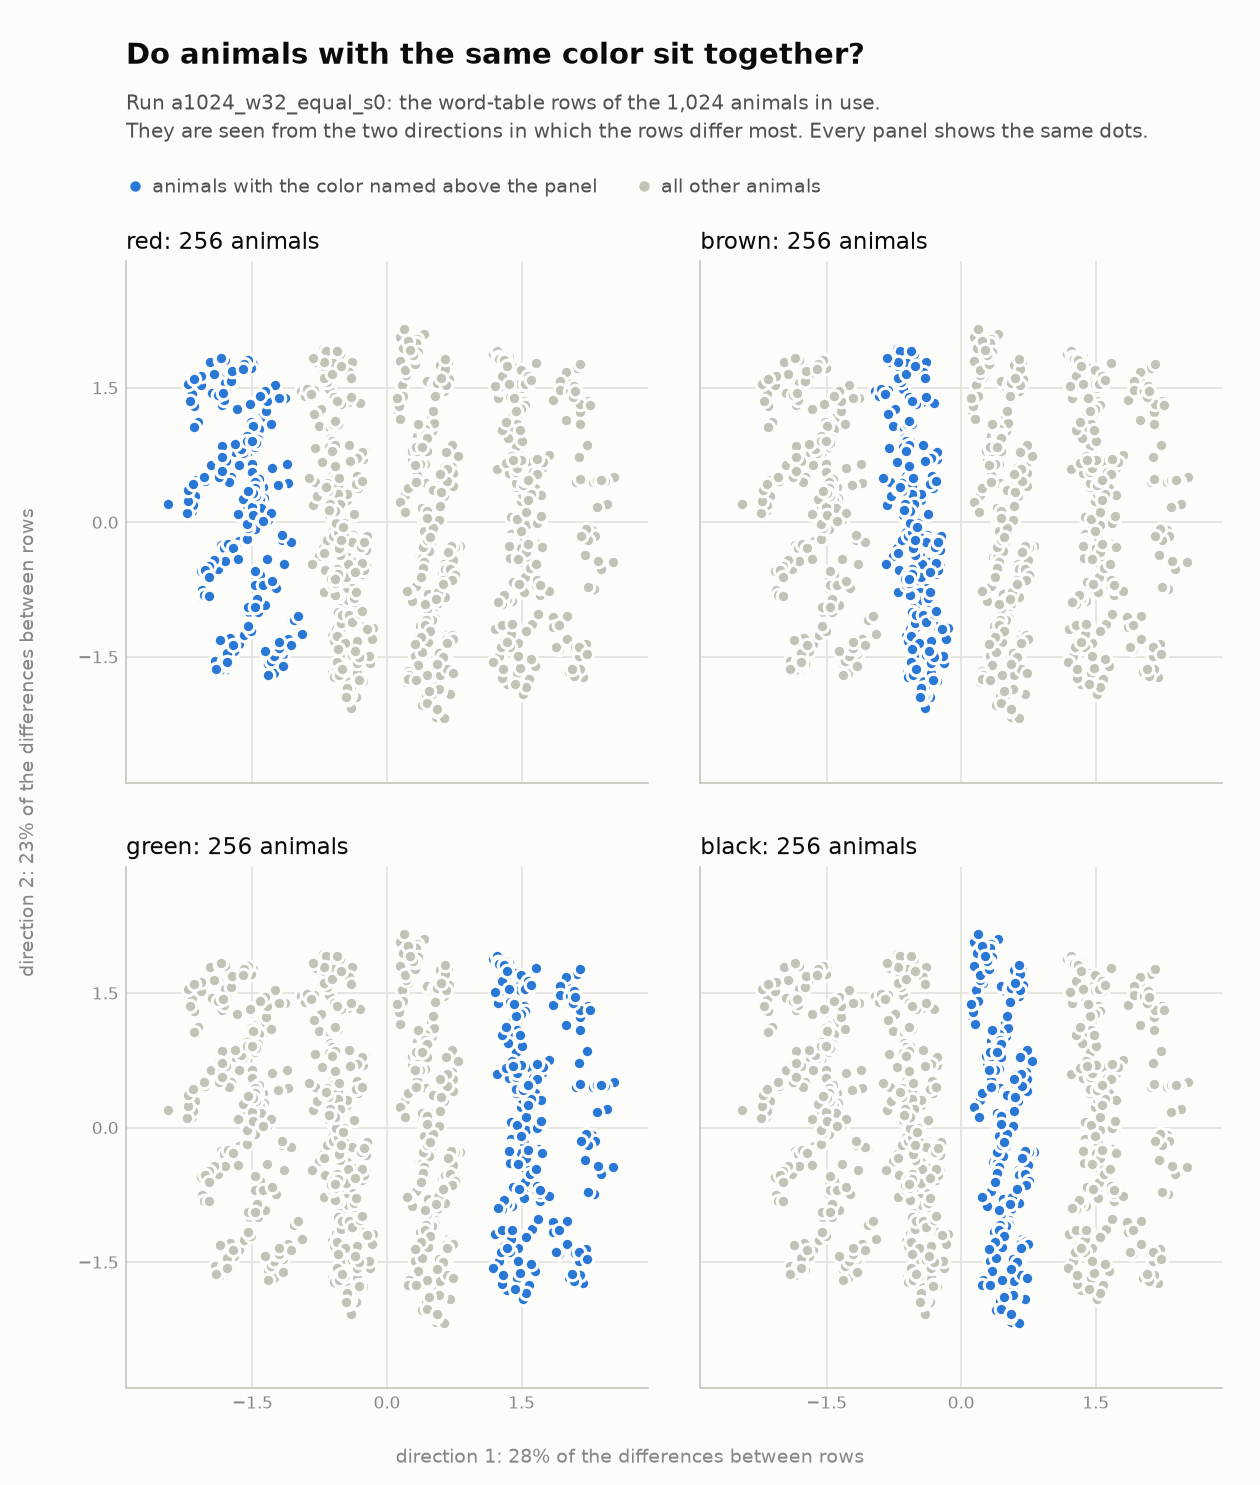
\includegraphics[width=0.44\textwidth]{figures/probe_a1024_w32_equal_s0_color.png}
\caption{The rows of the 1,024 animals in one model of width 32. A row has 32 numbers, too many
to draw. So each row is squeezed down to two numbers, each a weighted sum of the 32, chosen as
the two sums that vary most from one animal to another. Each dot is one animal, placed by those
two numbers, and animals with similar rows land close together. The four panels show the same
dots; each highlights the animals of one color. They fall into four bands.}
\label{fig:probe}
\end{figure}

This supports the claim your idea starts from: in these models an animal's row is, to a large
extent, a description of what the word means. Part of this could not have come out otherwise.
The row is the only thing that tells the model one animal from another, so a model that knows
every fact must be holding the facts in the rows somehow. What we learn is how: animals that
mean the same get nearly the same row, and most of the meaning can be read out by a very
simple test. This result says nothing yet about size, that is, about whether a model that is
too small for its language does worse.
